\section{Modelo de comportamiento del módulo Aplicación Móvil}

La figura \ref{fig:casosUso:Aplicacion} muestra los casos de uso que integran la funcionalidad del módulo Aplicación Móvil en donde se visualiza el historias de lecturas de los signos vitales medidos por el sistema embebido así como las funciones agregar, consultar, editar y eliminar información del paciente que utilice el sistema.
%
\begin{figure}[htpb!]
	\begin{center}
		\fbox{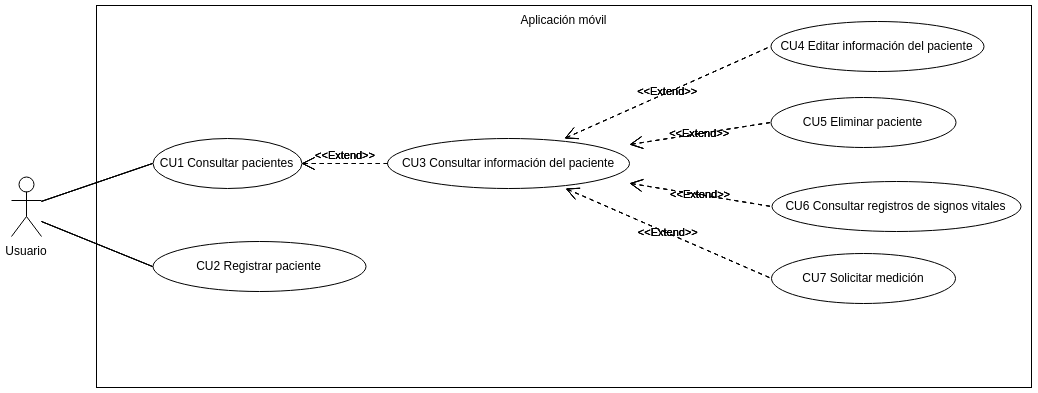
\includegraphics[width=0.9\textwidth]{ModeloComportamiento/imagenes/CasosUso_Usuario.png}}
		\caption{Diagrama de casos de uso del módulo Aplicación Móvil. \label{fig:casosUso:Aplicacion}}
	\end{center}
\end{figure}
\clearpage

\section{Modelo de comportamiento del módulo Sistema Embebido}

La figura \ref{fig:casosUso:sistema} muestra los casos de uso que integran la funcionalidad del módulo Sistema Embebido en el cual se realiza la medición, procesamiento y envío de los valores de los signos vitales en el paciente.

\begin{figure}[htpb!]
	\begin{center}
		\fbox{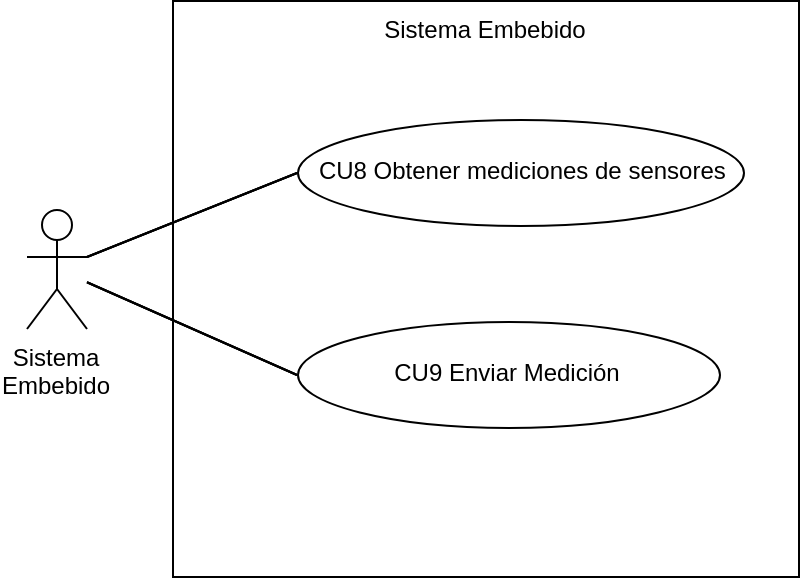
\includegraphics[width=0.4\textwidth]{ModeloComportamiento/imagenes/CUSistema.png}}
		\caption{Diagrama de casos de uso del módulo Sistema Embebido. \label{fig:casosUso:sistema}}
	\end{center}
\end{figure}
	
	\clearpage
	\pagebreak